\documentclass{beamer}
\usepackage[magyar]{babel}
\usepackage{t1enc}
\frenchspacing
\usepackage[utf8]{inputenc}
\usepackage{mathtools}
\usepackage{amsthm}
\usepackage{amsmath}
\usepackage{tikz}
\usepackage{graphicx}
\usepackage{xcolor}
\usepackage{listings}
\usepackage{graphicx}
\usetikzlibrary{matrix}
\theoremstyle{definition}
\newtheorem{defin}{Definíció}
\newtheorem{tet}{Tétel}
\usetheme{Dresden}
\usefonttheme{structuresmallcapsserif}
\usecolortheme{seagull}
\useinnertheme[shadow=true]{}
\usecolortheme{whale}
\usepackage{hyperref}
\usepackage{media9}

\newcommand{\includemovie}[3]{
\includemedia[%
  width=\linewidth,
  height=\linewidth,
activate=pagevisible,
deactivate=pageclose,
addresource=video.mp4,
flashvars={
src=video.mp4
&autoPlay=true 
&loop=true
&controlBarAutoHideTimeout=0 
}
]{}{StrobeMediaPlayback.swf}
}
\title{A matematika megoldatlan problémáinak listája}
\author{Nádpataki-Sass Bálint}
\date{\today}
\institute{Miskolci Egyetem}


\begin{document}
\maketitle

\begin{frame}{Tartalomjegyzék}
\tableofcontents
\end{frame}

\section{Bevezetés}

\begin{frame}{Bevezetés}

\transdissolve

    A matematikának, mint minden tudományterületnek léteznek mind a mai napig megoldásra váró problémái. A tudományág problémáinak egyedisége abban rejlik, hogy nem szükséges a tanulmányozásukhoz különösebb felszerelés vagy terepmunka, ennek megfelelően néha zavarba ejtő irányból kapunk választ. Általában azonban elmondható, hogy a tanulmányozásukhoz szükséges a matematikában mint tudományágban való igen komoly elmélyedés.
    \begin{itemize}
        \pause
        \item Hosszú idő után megoldott problémák
        \pause
        \item Eddig megoldatlanok
    \end{itemize}
\end{frame}
\section{Nevezetes problémák}
\subsection{Lista}
\begin{frame}{Nevezetes problémák}
\transblindshorizontal
\begin{itemize}
    \item Hosszú idő után megoldott problémák
    \begin{itemize}
        \item Nagy Fermat-tétel
        \item Tökéletes számok
        \item Párhuzamossági axióma
        \item Waring-probléma
        \item Négyszín-tétel
    \end{itemize}
    \item Eddig megoldatlanok
    \begin{itemize}
        \item Riemann-sejtés
        \item Goldbach-sejtés
        \item Collatz-sejtés
            \begin{itemize}
                \item Mersenne-prímek
                \item Birch és Swinnerton-Dyer-sejtés
            \end{itemize}
    \end{itemize}
\end{itemize}
\end{frame}
\section{Megoldott problémák}
\subsection{Nagy Fermat-tétel}
\begin{frame}{Nagy Fermat-tétel}
\transblindsvertical
   Lehetetlen egy egész szám másodiknál nagyobb hatványát két ugyanannyiadfokú hatvány összegére bontani, és emellett még azt is állította, hogy ezt be tudja bizonyítani, csak „kevés a margó, semhogy befogadná”. Fermat sejtésének némiképp formálisabb megfogalmazása a következő:

    \begin{itemize}
        \pause
         \uncover<2->{
        \begin{block}{Tétel}
            Az $a^n + b^n + c^n$ diofantoszi egyenletnek nincs megoldása 2-nél nagyobb egész n esetén a nemnulla egész számok körében. 
        \end{block}
    }
        \pause
        \item Természetesen n = 2-re az egyenletnek megoldásai a pitagoraszi számhármasok.
    \end{itemize}
\end{frame}

\subsection{Waring-probléma}
\begin{frame}{Waring-probléma}

A Waring-probléma az additív számelmélet egyik alapfeladata, azzal foglalkozik, hogy hány darab k-adik hatvány (nem negatív egész szám k-adik hatványa) szükséges egy tetszőleges pozitív egész összegként való előállításához. Itt k egynél nagyobb egész. 
\end{frame}

\begin{frame}{Waring-probléma}

    \begin{center}\begin{exampleblock}{Példa}
            \[
g(k) \geq 2^{k} + \left\lfloor \left({\frac{3}{2}}\right)^{k} \right\rfloor - 2
\] ahol $\lfloor x \rfloor$ az x szám alsó egészrészét jelöli.

Ez a korlát úgy adódik, hogy mutatunk egy számot, aminek az előállításához legalább ennyi k-adik hatvány szükséges. Legyen
\[
r = \left\lfloor \left( \frac{3}{2} \right)^{k} \right\rfloor.
\]
        \end{exampleblock}
    \end{center}
\end{frame}
\subsection{Tökéletes számok}
\begin{frame}{Tökéletes számok}
    \begin{figure}
    \centering
    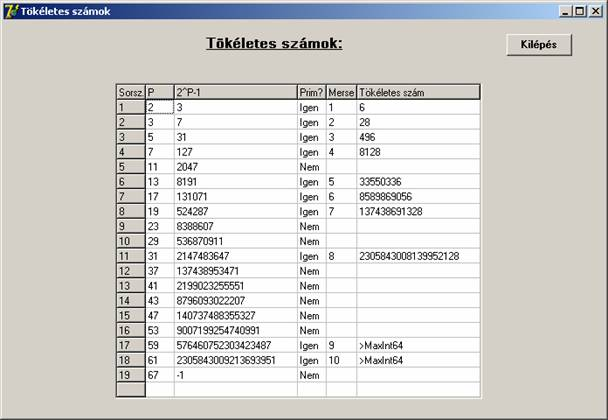
\includegraphics[width=0.6\textwidth]{tokeletesszamok.jpg}
    \caption{Tökéletes számok keresése}
\end{figure}
\end{frame}

\subsubsection{Tökéletes számok keresése Pythonban}
\begin{frame}{Tökéletes számok keresése Pythonban}
    \lstinputlisting[language=Python]{perfectnumber.py}
\end{frame}


\section{Máig megoldatlan problémák}
\subsection{Fermat-prímek}
\begin{frame}{Fermat-prímek}
\transsplitverticalin
    \begin{itemize}
        \item[]    Olyan Fermat-számok, amelyek prímek; tehát $Fn=2^{2^n+1}$ alakú prímszámok. Összesen öt ismeretes: F0=3, F1=5, F2=17, F3=257, F4=65537. Fermat felállította azt a sejtést, hogy minden ilyen alakú szám prímszám.
            \pause
        \item[]Bizonyos heurisztikus érvelések alapján általánosan elfogadott az a vélemény, hogy nincs több Fermat-prím.
    \end{itemize}
    \begin{table}[h]
  \centering
  \begin{tabular}{|c|c|}
    \hline
    \textbf{Index} & \textbf{Érték} \\
    \hline
    $F_0$ & 3 \\
    $F_1$ & 5 \\
    $F_2$ & 17 \\
    $F_3$ & 257 \\
    $F_4$ & 65537 \\
    \hline
  \end{tabular}
\end{table}
\end{frame}

\subsubsection{Prímszámok}
\begin{frame}{Prím számok}
\begin{table}[h]
  \centering
  \caption{Az első 10 prímszám}
  \begin{tabular}{|c|c|}
    \hline
    \textbf{Index} & \textbf{Prímszám} \\
    \hline
    1 & 2 \\
    2 & 3 \\
    3 & 5 \\
    4 & 7 \\
    5 & 11 \\
    6 & 13 \\
    7 & 17 \\
    8 & 19 \\
    9 & 23 \\
    10 & 29 \\
    \hline
  \end{tabular}
\end{table}
\end{frame}

\subsubsection{Videó Fernat-prímekről}
\begin{frame}{Videó Fernat-prímekről}
\begin{center}%
    \includemovie{\textheight}{\textheight}{video.mp4}
\end{center}
\end{frame}

\subsection{Ikerprím-sejtés}
\begin{frame}{Ikerprím-sejtés}
Ikerprím-sejtésnek nevezik azt a sejtést, hogy végtelen sok olyan p prímszám van, amire p+2 is prím. (Mint például 3,5; 5,7; 11,13; 17,19.) A sejtést először Eukleidész fogalmazta meg i. e. 300 körül.
\end{frame}

\section{Forrásjegyzék}
\begin{frame}{Forrásjegyzék}
\transsplitverticalin
\begin{thebibliography}{9}
    \bibitem{latex-beamer}
        \href{https://t.ly/aZ1St}{Wikipedia: A matematika megoldatlan problémáinak listája}.
    \bibitem{latex-beamer}
        \href{https://shorturl.at/nsDM6}{Wikipedia: Nagy Fermat-tétel}.
    \bibitem{latex-beamer}
        \href{https://shorturl.at/doPQX}{Wikipedia: Wikipedia: Waring-probléma}.
    \bibitem{latex-beamer}
        \href{https://shorturl.at/cmAK0}{Wikipedia: Tökéletes számok}.
    \bibitem{latex-beamer}
        \href{https://shorturl.at/bkRT4}{ Wikipedia: Fermat prímek}.
    \bibitem{latex-beamer}
        \href{https://shorturl.at/cFJW1}{Wikipedia: Ikerprím-sejtés}.
    
\end{thebibliography}
\end{frame}



\end{document}